% =============================================================================
%  Irradiation Studies and Design Optimization of the ATLAS Tile Calorimeter
%  for the High-Luminosity LHC
%
%  Author:  Róbert Astaloš, on behalf of the ATLAS Tile Calorimeter System
%  Style:   tikzposter, A0 portrait, ATLAS colour scheme
%
%  Figures (build/assets/):
%    fig_minidrawer_blockdiagram.png   Valdes 2023 JINST, Fig.1
%    fig_db6_blockdiagram.png          Valdes 2023 JINST, Fig.2
%    fig_db6_tid_test.png              Valdes 2023 JINST, Fig.3
%    fig_mosfet_threshold.png          Valdes 2023 JINST, Fig.4
%    fig_radiation_criteria.pdf        Moayedi TWEPP2025
%    fig_lvps_brick.pdf                Moayedi TWEPP2025
%    fig_wire_reduction.pdf            Moayedi TWEPP2025
%    fig_lvps_tests_overview.pdf       Moayedi TWEPP2025
%  Logo (build/logos/): atlas_transparent.png
%
%  Compile:  pdflatex newest-poster.tex   (run twice for references)
% =============================================================================

\documentclass[a0paper,portrait, blockverticalspace=4em, colspace=2em]{tikzposter}
\tikzposterlatexaffectionproofoff
\usepackage{graphicx}
\usepackage{amsmath}
\usepackage{amssymb}
\usepackage{hyperref}
\usepackage{multicol}
\usetikzlibrary{calc}

% ---------------------------------------------------------------------------
%  Colours — do not change; must match ATLAS colour scheme
% ---------------------------------------------------------------------------
\definecolor{maincolor}{HTML}{9e2b2f}
\definecolor{secondarycolor}{RGB}{158, 43, 47}
\definecolor{lightred}{RGB}{237, 199, 201}

% Radiation-effect callout colours — use these macros in prose, never raw hex
\definecolor{tid}{RGB}{254,128,2}   % orange  — Total Ionizing Dose
\definecolor{niel}{RGB}{0,140,0}    % green   — Non-Ionizing Energy Loss
\definecolor{see}{RGB}{190,0,62}    % red     — Single Event Effects
\definecolor{sel}{RGB}{0,90,170}    % blue    — Single Event Latch-up

% ===========================================================================
%  LAYOUT PARAMETERS — find and adjust all style knobs here.
%  After any change: cd build && ./build.sh newest-poster.tex
%  The change is not done until check_fit.py prints "RESULT: PASS".
% ===========================================================================
%
%  1. Inter-card vertical gap (white space between bottom of one card and
%     top of the next). MUST be set in \documentclass on line 22.
%     Current value: 4em  — increase for more breathing room.
%
%  2. Body text font size — controlled by \looseitems / \tightitems below.
%     Currently: \small (same as the References card).
%     Options: \normalsize (larger) | \small | \footnotesize (smaller)
%
%  3. Caption font size & leading — controlled by \captiontext below.
%     Currently: \footnotesize, baselinestretch=0.88 (12% tighter than normal).
%
%  4. List item spacing:
%     col1/col3 (loose):  itemsep=0.3em   — edit in \looseitems below
%     col2 (tight):       itemsep=0.15em  — edit in \tightitems below
%
%  5. Minimum figure width: 0.90\linewidth (design rule — do not go below).
%
% ---------------------------------------------------------------------------
%  Body text — \small = same size as References card.
%  Use \looseitems in col1/col3, \tightitems in col2 (col2 overflows first).
% ---------------------------------------------------------------------------
\newcommand{\looseitems}{\small\begin{itemize}\setlength{\itemsep}{0.3em}}
\newcommand{\tightitems}{\small\begin{itemize}\setlength{\itemsep}{0.15em}}

% ---------------------------------------------------------------------------
%  Caption style — \footnotesize + 12\% tighter leading.
%  All figure/table/graph captions call \captiontext{...}.
% ---------------------------------------------------------------------------
\newcommand{\captiontext}[1]{%
    {\footnotesize\renewcommand{\baselinestretch}{0.88}\selectfont#1}}

% ---------------------------------------------------------------------------
%  Theme
% ---------------------------------------------------------------------------
\usetheme{Default}
\definecolorstyle{atlascolors}{
    \colorlet{backgroundcolor}{white}
    \colorlet{titlefgcolor}{white}
    \colorlet{titlebgcolor}{maincolor}
    \colorlet{blocktitlefgcolor}{white}
    \colorlet{blocktitlebgcolor}{maincolor}
    \colorlet{blockbodyfgcolor}{black}
    \colorlet{blockbodybgcolor}{lightred!25}
}{}
\usecolorstyle{atlascolors}

% Title bar with ATLAS logo at right
\definetitlestyle{sampletitle}{width=760mm, roundedcorners=20, linewidth=2pt,
  innersep=10pt, titletotopverticalspace=6mm, titletoblockverticalspace=8mm}{%
  \begin{scope}[line width=\titlelinewidth, rounded corners=\titleroundedcorners]
    \draw[color=blocktitlebgcolor, fill=titlebgcolor]
      (\titleposleft,\titleposbottom) rectangle (\titleposright,\titlepostop);
  \end{scope}
  \node[anchor=east, fill=white, rounded corners=10pt, inner sep=10pt, xshift=-22mm]
    at ($(\titleposright,\titlepostop)!0.5!(\titleposright,\titleposbottom)$)
    {
\includegraphics[height=8.6cm]{logos/atlas_transparent.png}};}
\usetitlestyle{sampletitle}

\title{\parbox{0.74\linewidth}{\centering\huge
    Irradiation Studies and Design Optimization of the\\[2mm]ATLAS Tile Calorimeter for the High-Luminosity LHC}}
\author{Róbert Astaloš \quad on behalf of the ATLAS Tile Calorimeter System}
\institute{Comenius University Bratislava}
\date{}

\setlength{\columnsep}{0.5cm}

\begin{document}
\maketitle

\begin{columns}

% ===========================================================================
%  COLUMN 1 — Context, read-out chain, radiation requirements
% ===========================================================================
\column{0.333}

\block{The ATLAS Tile Calorimeter \& the HL-LHC Upgrade}{
    \looseitems
        \item As the primary hadronic sampling calorimeter of ATLAS, TileCal
        (built from steel absorbers and scintillating plastic tiles, covering $|\eta|<1.7$)
        is crucial for measuring hadronic jets, missing transverse energy,
        hadronically decaying $\tau$-leptons, and for muon identification.
        \item To cope with the unprecedented instantaneous luminosity and pile-up
        of the \textbf{High-Luminosity LHC}, the entire on-detector electronics system
        is being \textbf{fully replaced}. This upgrade enables fully continuous,
        un-triggered digital read-out of all channels at \textbf{40\,MHz} with
        enhanced energy and timing resolution.
        \item This new hardware faces a vastly harsher radiation environment.
        Consequently, every single component must be rigorously qualified against
        \textbf{\textcolor{tid}{Total Ionizing Dose (TID)}},
        \textbf{\textcolor{niel}{Non-Ionizing Energy Loss (NIEL)}}, and
        \textbf{\textcolor{see}{Single Event Effects (SEE/SEL)}}.
    \end{itemize}
    \vspace{0.12cm}
    \begin{center}
        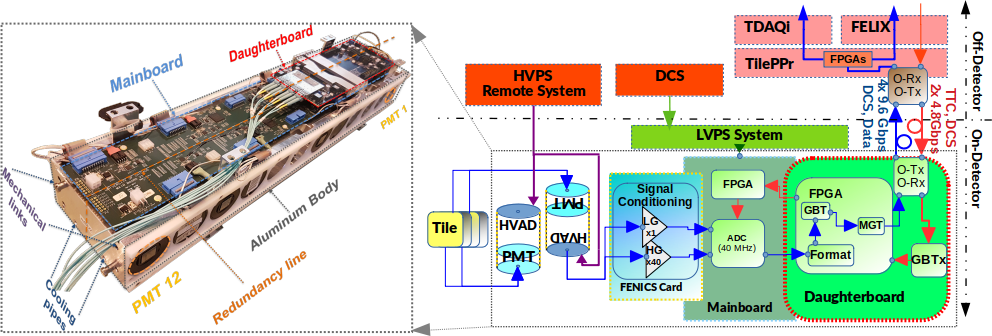
\includegraphics[width=0.98\linewidth]{assets/fig_minidrawer_blockdiagram.png}
    \end{center}
    \vspace{-0.2cm}
    \captiontext{TileCal Phase-II Minidrawer (left) and the on-/off-detector read-out
    chain (right).}
}

\block{Read-Out Chain \& Radiation Requirements}{
    \looseitems
        \item The on-detector electronics are partitioned into \textbf{896 Minidrawers (MDs)}.
        Each MD processes signals from up to 12 PMTs at 40\,MHz. The MD houses
        Front-End Boards (signal shaping), a \textbf{Mainboard (MB)} (digitization),
        and a \textbf{Daughterboard (DB)} (control, clock distribution, and high-speed data transmission).
        Power is supplied by the \textbf{Low-Voltage Power Supply (LVPS)}.
        \item Digital streams are transmitted off-detector via multi-Gbps optical links
        to FELIX and the Tile PreProcessor (TilePPr).
        \item Radiation criteria are based on ATLAS simulations for the
        \emph{most-exposed} regions, scaled by rigorous safety factors (SF):
        \textbf{1.5} (simulation uncertainty), $\mathbf{\times}$\textbf{3--5}
        (low-dose-rate effects / lot-to-lot variation),
        and \textbf{1.3} (non-monoenergetic beams).
        \item Final Daughterboard qualification targets (with all SFs applied):
        \textbf{\textcolor{tid}{TID $\approx$ 108\,Gy}},
        \textbf{\textcolor{niel}{NIEL $\approx 13.16\times10^{12}$\,n/cm$^2$}},
        \textbf{\textcolor{see}{SEE $\approx 4.54\times10^{11}$\,h/cm$^2$}}.
    \end{itemize}
    \vspace{0.12cm}
    \begin{center}
        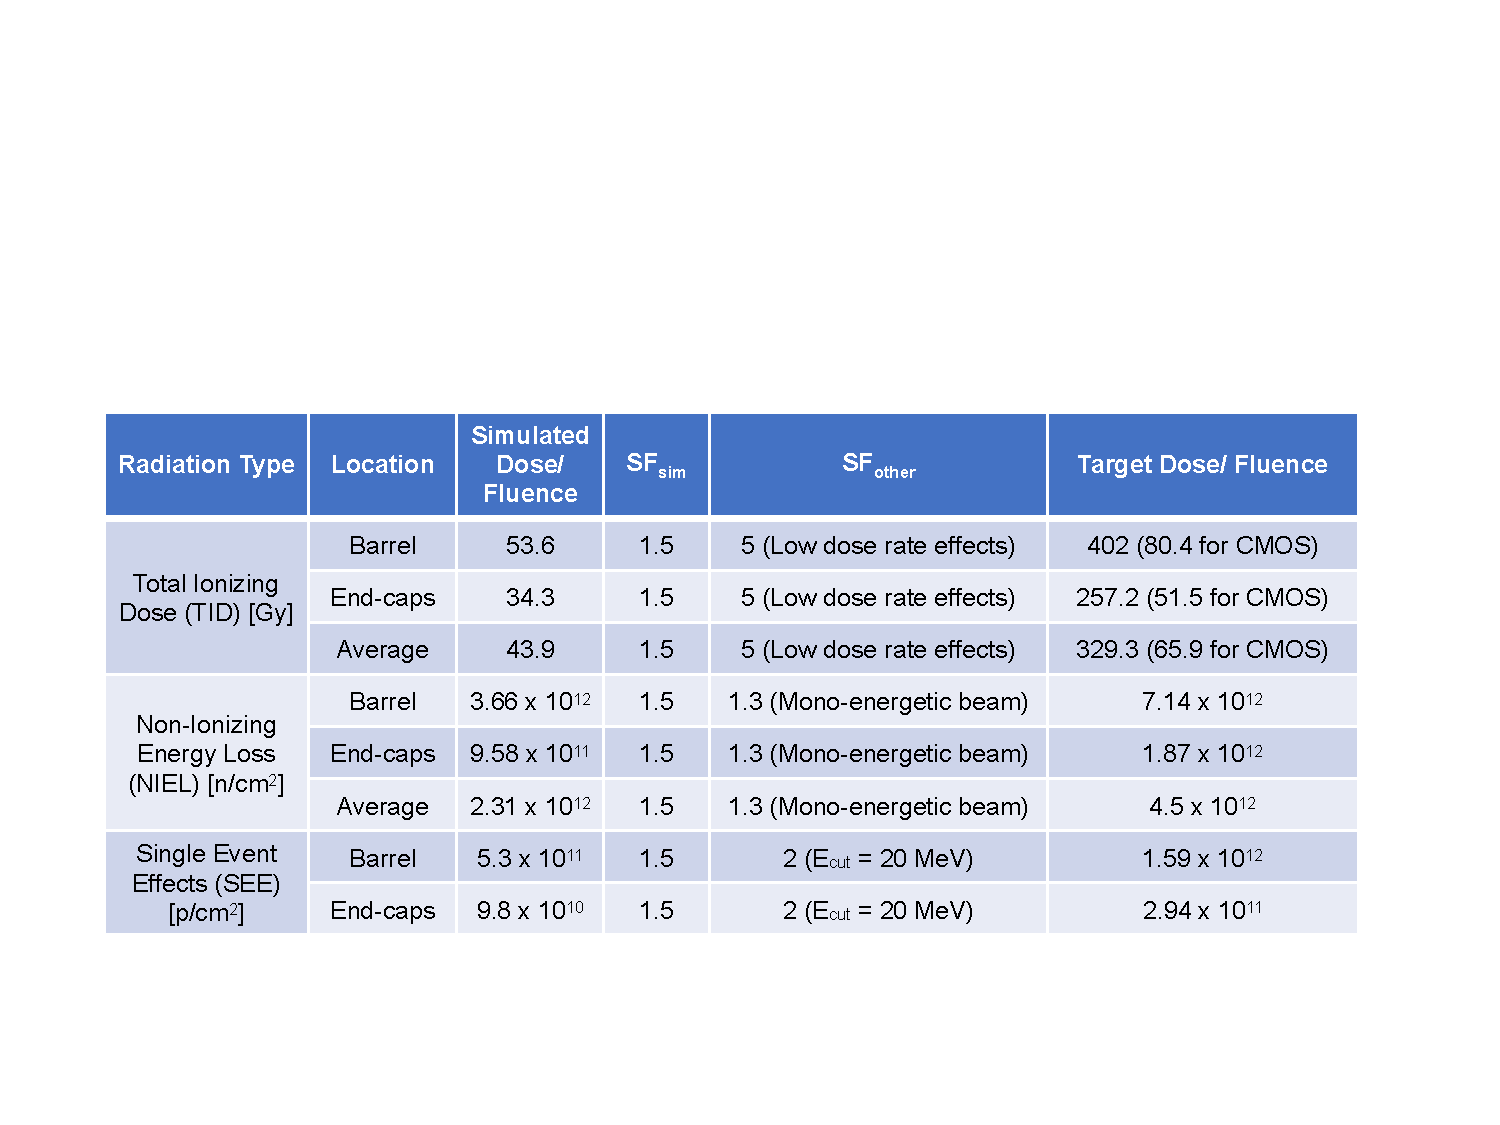
\includegraphics[width=0.99\linewidth]{assets/fig_radiation_criteria.pdf}
    \end{center}
    \vspace{-0.2cm}
    \captiontext{Worked example for the LVPS bricks: simulated dose/fluence scaled by
    safety factors to the qualification target.}
}

\block{References}{
    \small
    \begin{enumerate}\setlength{\itemsep}{0.2em}
        \item ATLAS Collaboration, \emph{Technical Design Report for the Phase-II
        Upgrade of the ATLAS Tile Calorimeter}, CERN-LHCC-2017-019, ATLAS-TDR-028 (2018).
        \item E. Valdes Santurio \textit{et al.}, \emph{Radiation studies performed
        on the High-Luminosity ATLAS TileCal link Daughterboard}, JINST \textbf{18}
        (2023) C04011.
        \item E. Valdes Santurio \textit{et al.}, \emph{Radiation studies on the
        ATLAS Link and Control Daughterboard for the HL-LHC Upgrade}, IEEE NSS MIC
        RTSD (2025).
        \item S. Moayedi (ATLAS), \emph{Upgrade of the ATLAS Tile Calorimeter
        Front-End Power Supply for the HL-LHC}, TWEPP 2025, ATL-TILECAL-SLIDE-2025-552.
    \end{enumerate}
}

% ===========================================================================
%  COLUMN 2 — Daughterboard irradiation studies
%  NOTE: figures are kept at 0.90\linewidth per design rule.
%        To fit three figure-heavy blocks, prose is kept to 2–3 tight bullets.
% ===========================================================================
\column{0.333}

\block{The Link \& Control Daughterboard (DB6)}{
    \tightitems
        \item The DB6 achieves exceptional radiation tolerance via a
        \textbf{double-redundant} A/B architecture enforced by
        \textbf{Triple Modular Redundancy (TMR)},
        \textbf{Xilinx Soft Error Mitigation (SEM)},
        \textbf{GBT-FEC} error correction, and \textcolor{sel}{SEL}-protection circuitry.
        \item Core components include 4$\times$ commercial \textbf{SFP+} transceivers
        (two 4.8\,Gbps downlinks, four 9.6\,Gbps uplinks), custom CERN
        \textbf{GBTx} ASICs, Xilinx \textbf{Kintex UltraScale (KU)}
        and Microsemi \textbf{ProASIC3} FPGAs.
    \end{itemize}
    \vspace{0cm}
    \begin{center}
        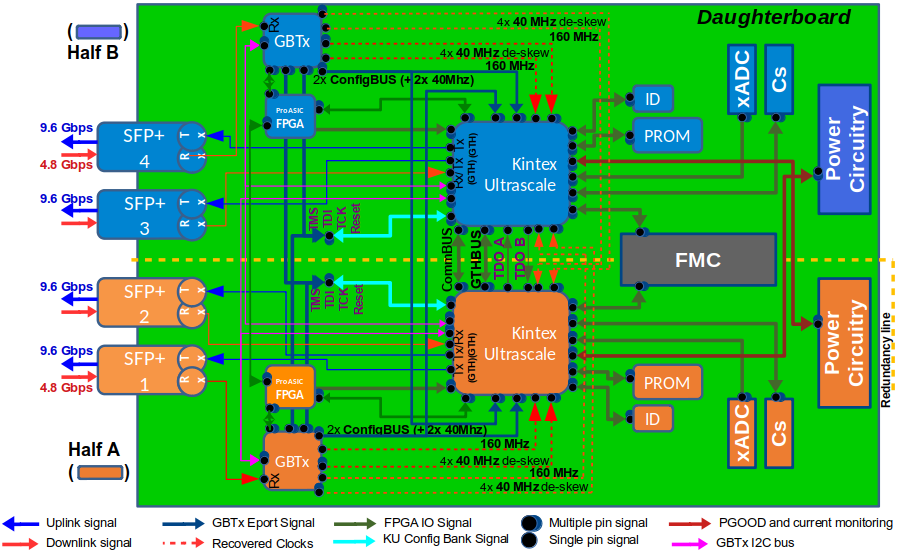
\includegraphics[width=0.90\linewidth]{assets/fig_db6_blockdiagram.png}
    \end{center}
    \vspace{-0.3cm}
    \captiontext{DB6 block diagram: two redundant halves, KU + ProASIC FPGAs, GBTx and
    four SFP$+$ optical links.}
}

\block{DB6 Radiation Qualification: TID, NIEL \& SEL}{
    \tightitems
        \item \textbf{\textcolor{tid}{TID}}: Boards irradiated at CERN CC60 ($^{60}$Co)
        to 220\,Gy at 3.37\,Gy/h and at IFJ Kraków (54\,MeV protons) to $\sim$400\,Gy
        at 2.88\,Gy/h. Temperatures and currents stable throughout — no TID damage.
        \item \textbf{\textcolor{niel}{NIEL}}: DB6-0 irradiated at the TRIGA reactor
        (JSI Ljubljana) to $14\times10^{12}$\,n$_\text{eq}$/cm$^2$. KU FPGAs showed
        strong tolerance; ProASIC and FLASH recovered after annealing.
        \item \textbf{\textcolor{sel}{SEL}}: Tests with 54\,MeV and 226\,MeV protons
        up to $1.11\times10^{12}$\,p/cm$^2$ yielded
        \textbf{zero single-event latch-ups} in all KU FPGAs.
    \end{itemize}
    \vspace{0cm}
    \begin{center}
        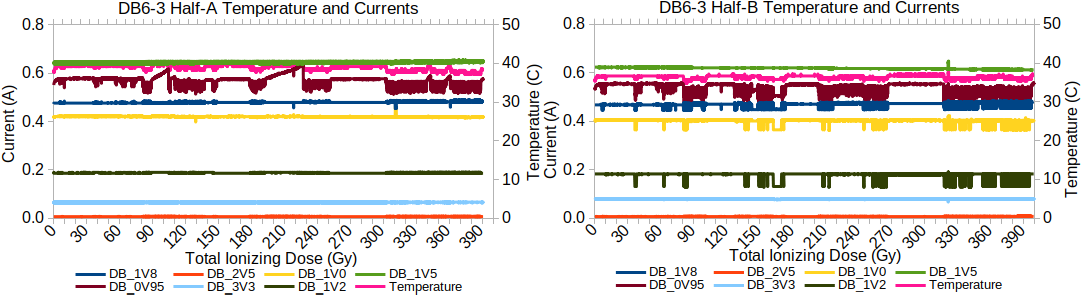
\includegraphics[width=0.90\linewidth]{assets/fig_db6_tid_test.png}
    \end{center}
    \vspace{-0.3cm}
    \captiontext{DB6-3 board currents and FPGA temperature, stable over the full
    $\sim$400\,Gy proton \textcolor{tid}{TID} run (both halves).}
}

\block{Component Results \& Production}{
    \tightitems
        \item \textbf{SFP$+$ Selection}: AVAGO modules failed; 1/9 CORETEK failed at
        $9\times10^{12}$\,n/cm$^2$. \textbf{Direktronik 33-4248} and
        \textbf{FS-Europe SFP-10GSR-85} passed and were selected.
        \item \textbf{Design Revisions}: FDFMA3N109 MOSFETs showed threshold shifts,
        removing the \textcolor{sel}{SEL} over-current circuit. 4/15 LTC6902
        oscillators failed and were eliminated. All essential components now
        qualified; $\sim$\textbf{930 DB6 units} to be produced in \textbf{2026--2027}.
    \end{itemize}
    \vspace{0cm}
    \begin{center}
        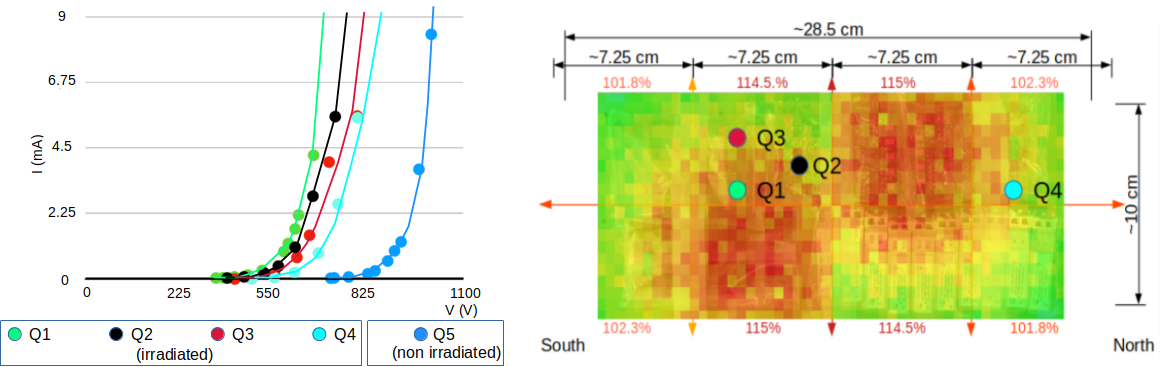
\includegraphics[width=0.90\linewidth]{assets/fig_mosfet_threshold.png}
    \end{center}
    \vspace{-0.3cm}
    \captiontext{FDFMA3N109 threshold shift (IV curves, left) correlated with the reactor
    cavity flux map (right).}
}

% ===========================================================================
%  COLUMN 3 — LVPS optimisation + conclusions
% ===========================================================================
\column{0.333}

\block{LVPS Bricks \& Design Optimisation}{
    \looseitems
        \item Located in the module \emph{fingers}, the LVPS experiences the most severe
        radiation environment within TileCal. The Phase-II design deploys \textbf{8 independent
        DC-DC ``bricks''} per module: each a 300\,kHz two-switch forward converter stepping
        \textbf{200\,V down to 10\,V} ($\sim$23\,W). This segmentation boosts reliability
        and isolates localised failures.
        \item \textbf{Enhanced Efficiency}: Replacing the STB57N65M5 MOSFET with
        \textbf{SIHFS9N60A} improved brick efficiency from $\sim$58\% to \textbf{$\sim$72\%},
        surpassing the $\geq$65\% threshold set by the 77\,kW cooling plant.
        \item \textbf{Simplified Wiring}: Control signals halved from \textbf{18} to \textbf{9}
        via a tri-state logic scheme (on/off/hold), easing routing from the service cavern.
    \end{itemize}
    \vspace{0.1cm}
    \begin{center}
        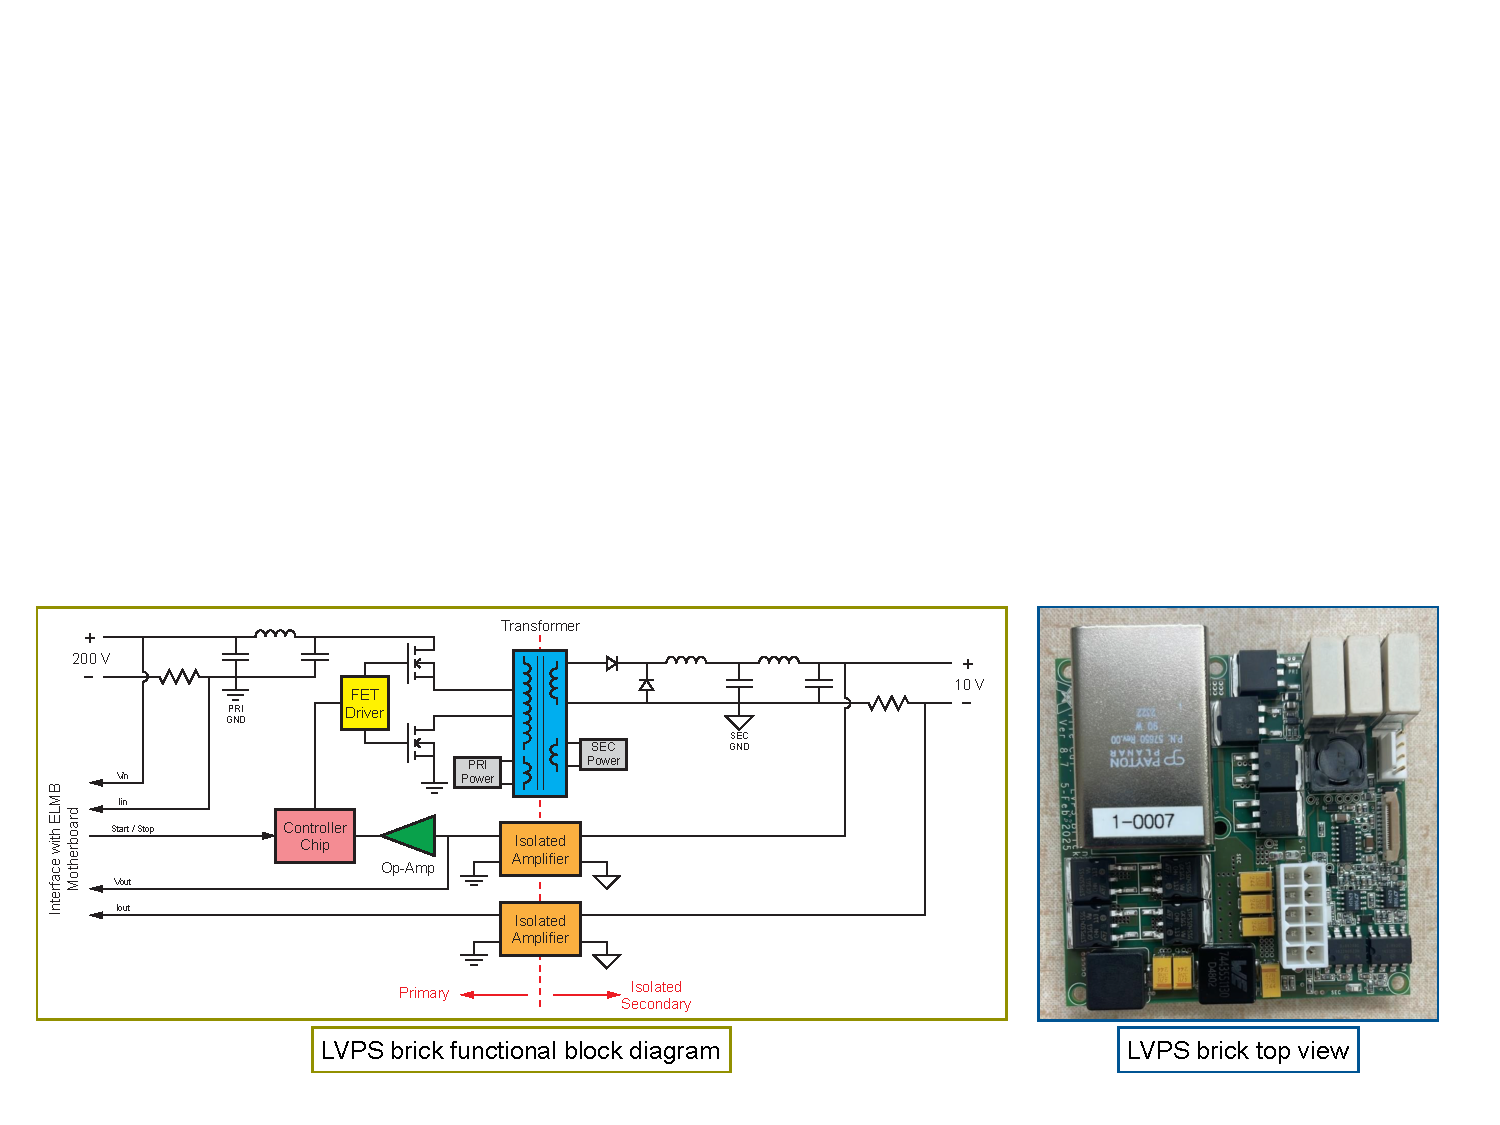
\includegraphics[width=0.90\linewidth]{assets/fig_lvps_brick.pdf}\\[2mm]
        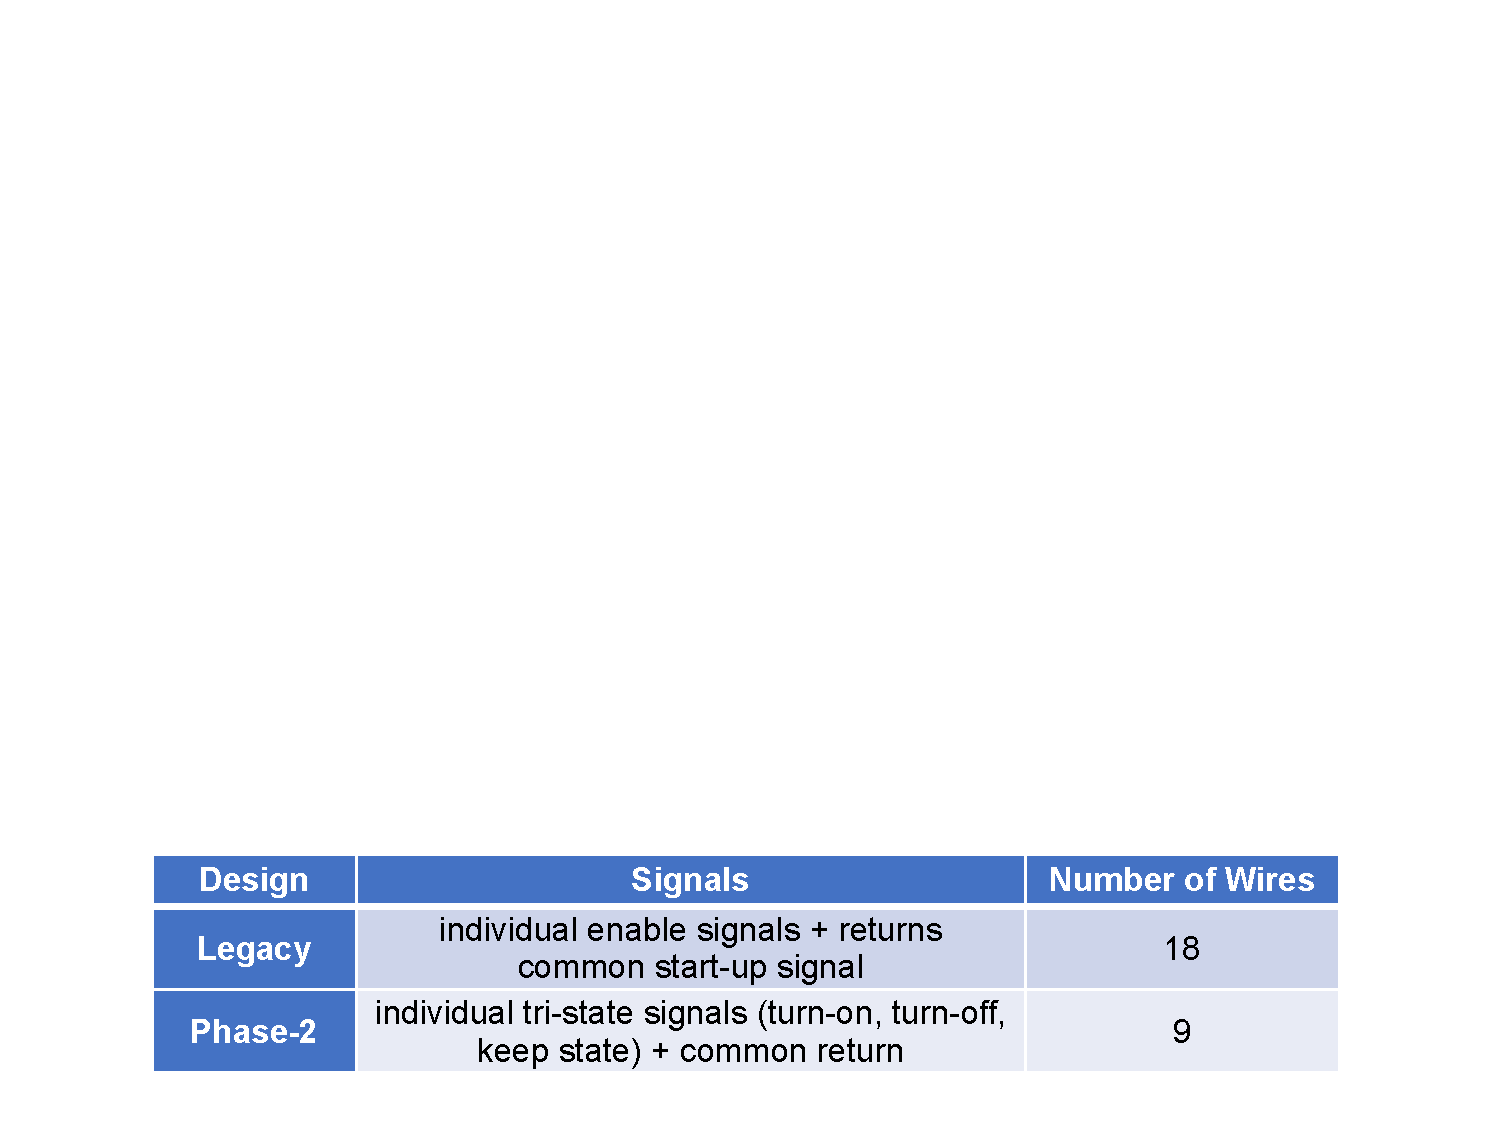
\includegraphics[width=0.90\linewidth]{assets/fig_wire_reduction.pdf}
    \end{center}
    \vspace{-0.3cm}
    \captiontext{LVPS brick diagram and top view (top); 18-to-9 control-wire reduction (bottom).}
}

\block{LVPS Radiation Qualification}{
    \looseitems
        \item Components tested for \textbf{\textcolor{tid}{TID}} (CC60/PSI),
        \textbf{\textcolor{niel}{NIEL}} (TRIGA), and \textbf{\textcolor{see}{SEE}} (PIF);
        assembled bricks validated in \textbf{system tests at CERN CHARM}.
        \item Critical parts (7 diodes, \textbf{LT1681}, \textbf{LTC6241},
        \textbf{LT3080}, \textbf{IR2110}, \textbf{SIHFS9N60A}) all passed with only minor shifts.
        \item \textbf{SI8920} isolation amplifier is stable when input $\leq$100\,mV;
        pre-production MOSFETs failed at 323\,Gy (well beyond the 80\,Gy req.);
        HCPL7800 failed at $2.75\times10^{12}$\,n/cm$^2$ — all dictated final selections.
    \end{itemize}
    \vspace{0.1cm}
    \begin{center}
        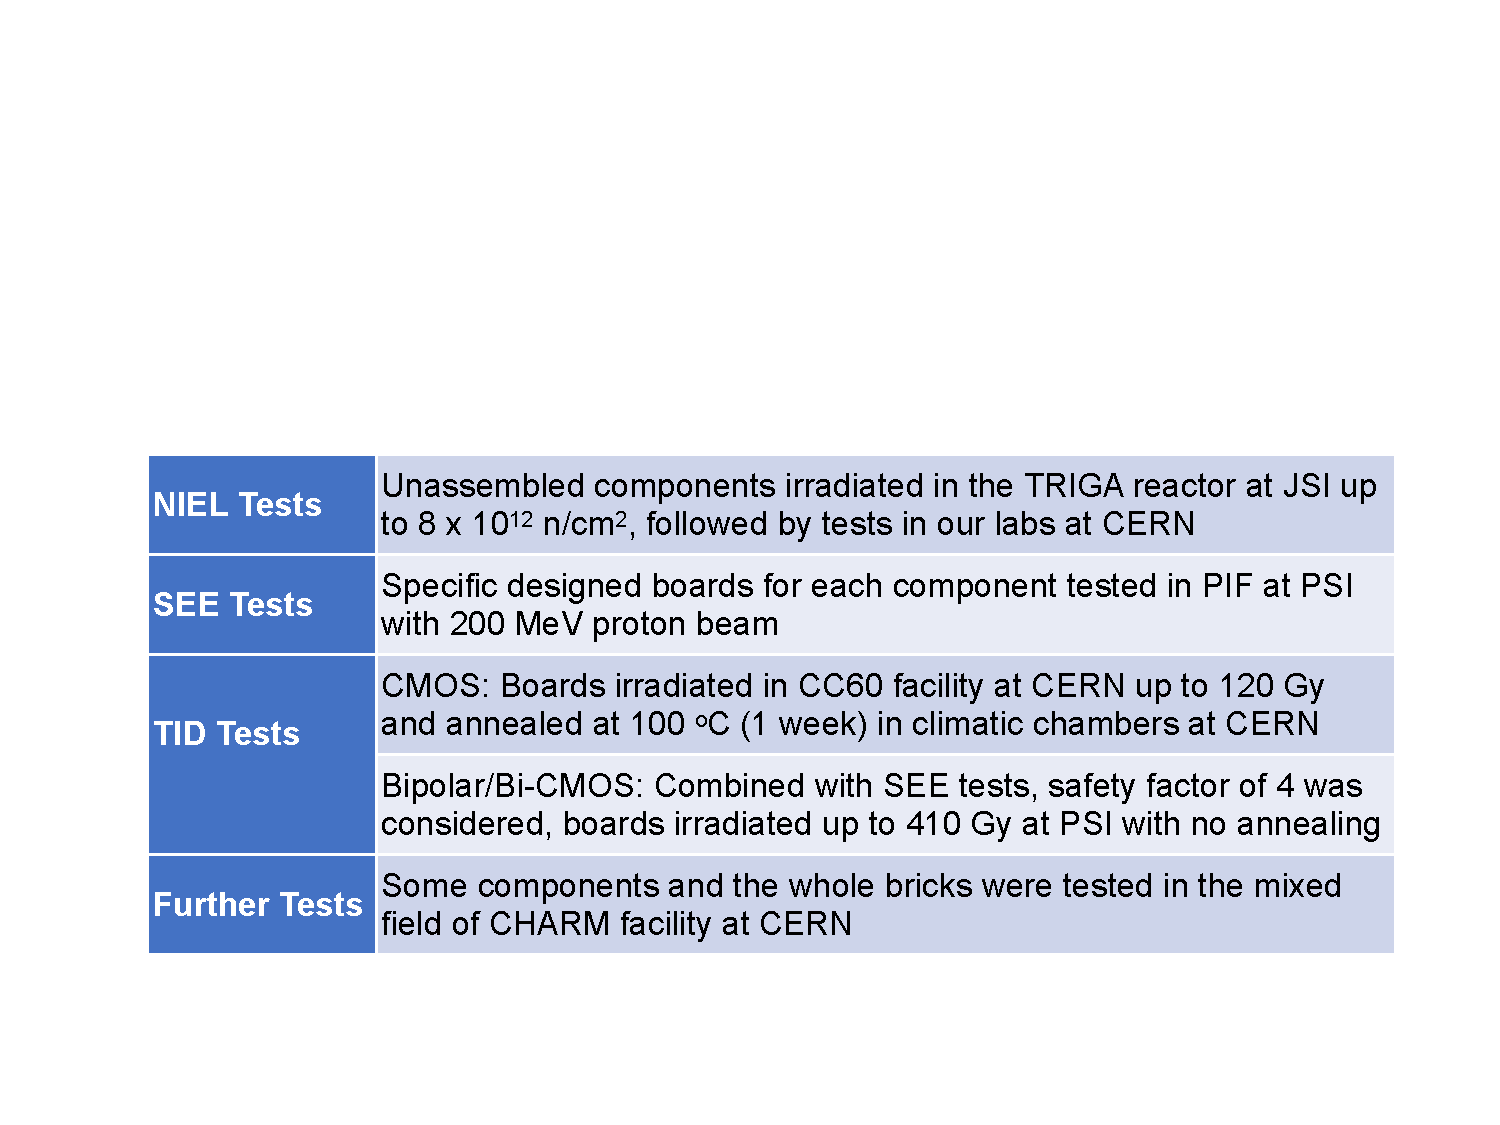
\includegraphics[width=0.90\linewidth]{assets/fig_lvps_tests_overview.pdf}
    \end{center}
    \vspace{-0.3cm}
    \captiontext{Irradiation campaign overview: facility and beam type per test category.}
}

\block{Conclusions \& Outlook}{
    \looseitems
        \item Both \textbf{LVPS bricks} and the \textbf{Link Daughterboard}
        successfully satisfy HL-LHC \textcolor{tid}{TID}, \textcolor{niel}{NIEL}, and
        \textcolor{see}{SEE} benchmarks.
        \item Radiation studies \textbf{directly drove design optimisation}: vulnerable parts
        were removed from the DB, while the LVPS gained improved efficiency
        ($\sim$58\%$\to$$\sim$72\%) and simplified wiring.
        \item \textbf{Project Outlook}: Mass production of $\sim$930 Daughterboards
        is slated for 2026--2027. Lot-acceptance testing proceeds through 2025--2026.
    \end{itemize}
}

\end{columns}
\end{document}
